\chapter{Background \& State of the art}
\label{chap3}

This chapter describes what glitch attacks are, why developers need to protect their devices from them and the current limitations related to this. The \textit{CV32E40S} RISC-V core by the OpenHW group is also introduced, and the potential benefits of replacing some of its security features are investigated. 

\section{What are glitch attacks?}
\label{sec:glitch_attacks}

Glitch attacks, also known as hardware fault injection, are a sophisticated form of hacking aimed at exploiting vulnerabilities in hardware systems. The primary objective is to disrupt normal execution to bypass security features in order to gain access to sensitive data, bypass authentication protocols or undermine cryptographic operations. 

Glitch attacks can be divided into two main categories: invasive (e.g., decapsulating the chip\cite{intro_to_hw_hacking}) and non-invasive attacks (e.g., electromagnetic fault injection (EMFI), voltage- and clock-glitching). Often times software and firmware security measures can only protect against non-invasive glitches, as protecting from invasive glitches often require hardware modifications\cite{glitchresistor}. Due to the nature of invasive attacks, it is beyond the scope of this project to defend against them. This is because these often aim at tampering with Read-Only Memory (ROM) or Boot-loaders on Printed Circuit Boards (PCBs), and are not effective against more complex systems like a Central Processing Unit (CPU) or a System on Chip (SoC). Therefore, protecting against these attacks is the responsibility of other components than the core.

\subsection{Non-invasine glitch attacks}
\label{sec:non_invasive}

Non-invasive glitches can be performed as long as an attacker has access to a device. However, there is quite a lot of procedural vulnerability discovery that has to be done before an attack can be performed\cite{arm_presentation_2}. In the case of Electromagnetic Fault Injection (EMFI) the chip has to be repeatedly exposed to electromagnetic interference during execution, to then determine which areas are most vulnerable to attacks\cite{emfi_injection}. An example of such probing having been performed on the BCM2837 SoC can be seen in \autoref{fig:emfi_map}\cite{emfi_injection}. 

Voltage- or clock-glitching can be performed as long as there is some way to access these signals externally. Voltage-glitching often requires the removal of power filtering capacitors to gain more fine-grained control over a processor's voltage input. However, both of these methods require very precise timing by an attacker. This is why specialized tools such as the \textit{ChipWhisperer}\cite{chipWhisperer} were made, as they allow for extremely accurate fault-injection. These days it is also possible to perform effective glitch attacks with simple components in conjunction with a cheap Field Programmable Gate Array (FPGA) which outputs precise triggers as shown by\cite{hole_in_soc}. 

\begin{figure}[h!]
    \centering
    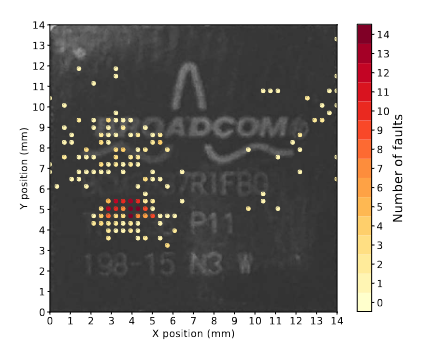
\includegraphics[scale=0.5]{docs/images/emfi_error_map.png}
    \caption{EMFI BCM2837 sensitivity map (dot size is not corralated with probe size.)\cite{emfi_injection}.}
    \label{fig:emfi_map}
\end{figure}

Voltage-glitching is performed by momentarily dropping the supply voltage during execution of critical operations. Clock-glitching is performed by altering clock timing to violate setup and hold time requirements of the hardware\cite{intro_to_FI}. The results of glitches cannot always be predicted, however they mainly result in skipped or repeated CPU instructions, incorrect evaluation of CPU instructions or corrupt reads from memory devices\cite{intro_to_FI}. In general these faults can occur at any stage in the execution pipeline. A typical application for these types of glitches is to skip some sort of signature verification in a bootloader or other security module. Take for instance the example code shown in \autoref{fig:glitchable_code}. This example shows an example of secure boot code. This is often a target for attacks as the execution time is deterministic, and given physical access to the device an attacker can try as many times as they want to bypass the authentication process \cite{arm_presentation}. 

In the code in \autoref{fig:glitchable_code} a boot image is first fetched. The result code of this operation is then checked to see whether the correct image was fetched, or if an error occurred. In the case of an error, the program is stuck in in an infinite loop. If the correct image was fetched the boot process can continue. From the figure we see that there exists a number of weak points that can be exploited using common forms of attacks. For example voltage- or clock-glitching could be used to bypass the 'boot\_go' function or jump out of the infinite while loop. EMFI and laser pulse attacks often offer a higher degree of spatial and temporal precision. This allows attacks to more effectively target specific pipeline stages, and could therefore be used to disrupt the conditional check or status registers\cite{intro_to_FI}. 

\begin{figure}[h!]
    \centering
    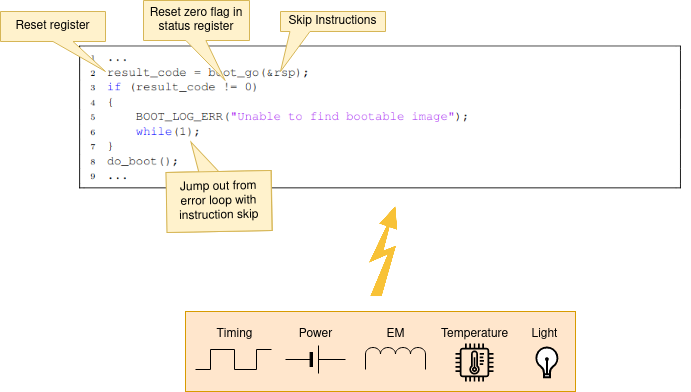
\includegraphics[width=0.75\textwidth]{docs/images/glitch_attack_whole_system.png}
    \caption{Example of code that can be glitched with common attacks. Figure inspired by one found in \cite{arm_presentation}.}
    \label{fig:glitchable_code}
\end{figure}

Because of this hardware designers often implement security features aimed at protecting against specific forms of attacks. This includes thins like \textit{Program Counter Hardening} (PCH) to check for instruction skips by comparing current and expected PC values, and \textit{Error Correcting Code} (ECC) to validate data integrity in registers\cite{cv32e40s_manual}. However, while these features would stop an attacker in this example, what if the attacker finds a way to boot with the wrong PC and start the program at the 'do\_boot' function? In this case we would need to develop a new form of protection with a greater fault detection coverage. Such a solution is investigated in this project in the form of a DCL mechanism in the \textit{CV32E40DC}. 

% Glitch attacks have over recent years become a more common and greater threat. Due to the nature of how these attacks are carried out, they are often a very affordable way to exploit hardware. Attackers have easy access to open source resources like the the 'ChipWhisperer Lite' which allows for easy access to hardware glitching tools as well as side channel analysis\cite{chipWhisperer}. In addition to this, FPGAs can be used to inject precisely timed faults as long as an attacker has access to the supply voltage or clock on a chip\cite{hole_in_soc}. 

\section{The need for glitch protection}
\label{sec:need}

Within the world of CPU design the two biggest architectures are ARM and x86 (produced by Intel and AMD). Most of the devices we use every day has one of these types of chips inside them, and because of this they also implement several security features to prevent glitch attacks. For ARM processors this includes, among other things, the \textit{TrustZone} which provides hardware-enforced isolation between trusted and non-trusted software, as well as built in physical attack protection\cite{arm}. The 12th generation x86 processors produced by Intel have a Tunable Replica Circuit (TRC), which uses hardware-based sensors to explicitly detect circuit-based timing failures that occur as the result of an attack\cite{intel}.  

Unfortunately, for many years the details of CPU design have been hidden from the public due to the strict secrecy producers have around their products\cite{riscv_wiki}. While this limits what the public can know, it also means that a potential hacker would have a much harder time finding exploits in the architecture. However, due to the nature of open source projects, this is a larger vulnerability for products based on the RISC-V instruction set architecture (ISA). An example of direct exploitation of the ISA was shown during the 'DEFCON' conference in 2019\cite{isa_exploit}. Here it was demonstrated that triggering an exception during boot of a RISC-V chip would lead to an 'exception loop'. This was because the Machine Trap Vector (MTVEC) had no base address before boot (e.g., it was set to 0x0). Pointing to this address is permitted in the ISA, and doing so will trigger an exception. This means that triggering an exception before boot leads to the exception handler pointing to an illegal address, which again triggers an exception and this continues forever. Handling of exceptions happens first at the highest privilege mode (Machine mode), which means that the chip is also stuck in this mode. The RISC-V architecture is designed with some key security features in mind. One of these are the previously mentioned privilege levels. These are in descending order: machine (M-mode), hypervisor (H-mode), supervisor (S-mode) and user mode (U-mode). A higher privilege mode can access all the functions used in a lower privilege mode\cite{source2}.

Other key security features in the RISC-V architecture are the physical memory protection (PMP), and the trusted execution environment (TEE). The PMP ensures that no access is given to protected parts of the memory region. The TEE is a secure and isolated area within a computer system that provides a higher level of security for processing sensitive information. One of the main objectives of the PMP and the privilege levels is to provide a TEE that isolates secure and insecure applications. It is critical for software and firmware developers that these features work. However, as shown in \cite{source2} the integrity of TEEs can be bypassed using clock-glitching. 

%\section{Previous Approaches to glitch protection}
\section{CV32E40S by the OpenHW group}
\label{sec:cv32}

The previously mentioned security measures of the RISC-V ISA do a decent job at protecting against glitch attacks, but as mentioned they can be bypassed. Therefore there is a need for more specialized security features. Because of this the \textit{OpenHW} group developed the \textit{CV32E40S}. This is a 4-stage in-order 32-bit RISC-V processor core with the main intention of ensuring secure operation\cite{cv32e40s_manual}. This core has the same privilege modes and PMP as described to ensure a TEE. There are however implemented extra security features through an Instruction Set Extension (ISE), \textit{Xsecure}. The CV32E40S started out as a fork of the CV32E40P which is another RISC-V processor made by the OpenHW group. The top-level block diagram of the CV32E40S core is shown in \autoref{fig:cv32e40s_block}. From the figure one can see that the architecture of this core is much like any other RISC-V core, with an Instruction Decode, Instruction Fetch, Execute and Write Back stage. 

%The extra security features of this core are a PCH module in the IF stage (not shown in figure), ECC in the register file in the ID and CSR Hardening in the EX stage. 

\begin{figure}[h!]
    \centering
    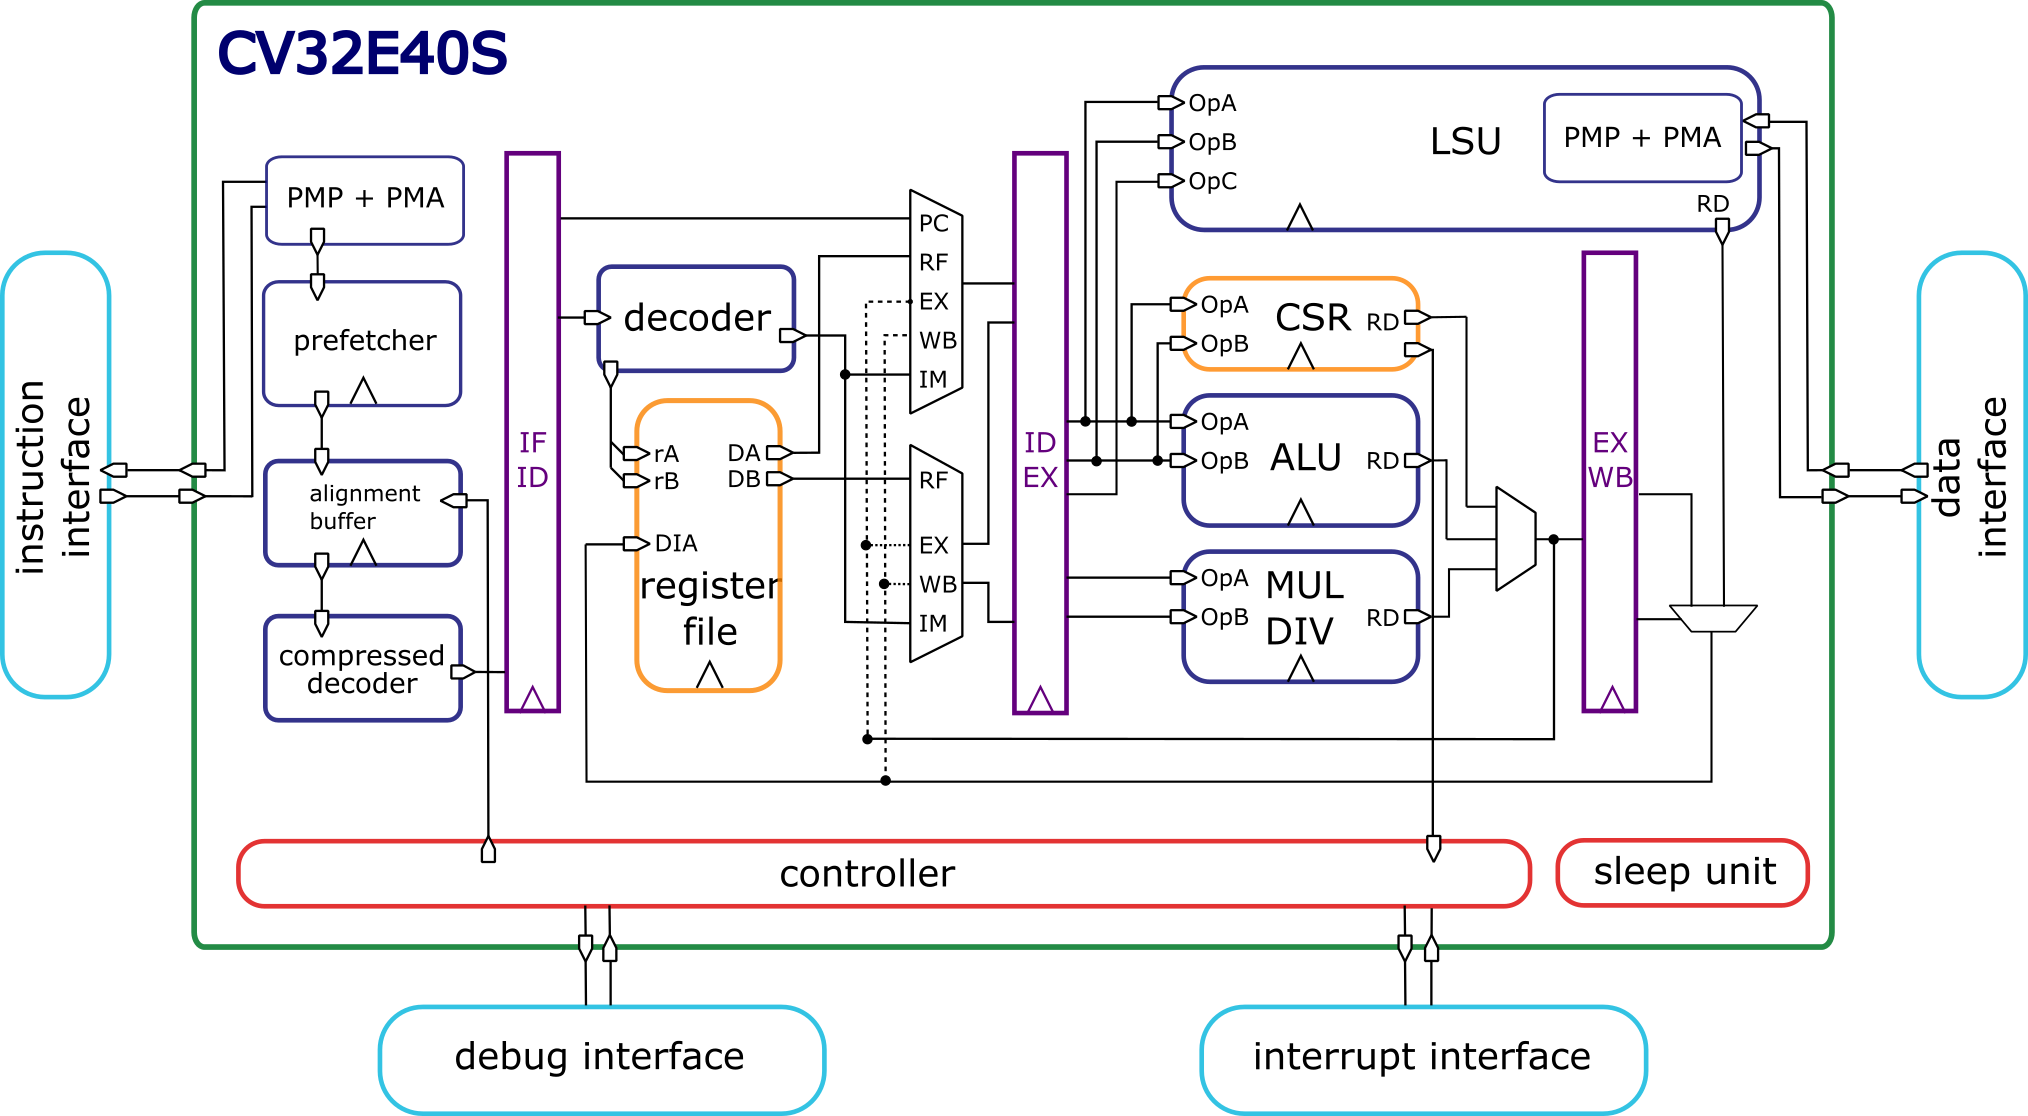
\includegraphics[width=0.8\textwidth]{docs/images/CV32E40S_Block_Diagram.png}
    \caption{CV32E40S top-level block diagram\cite{cv32e40s_manual}.}
    \label{fig:cv32e40s_block}
\end{figure}

\subsection{Xsecure Extension}
\label{sec:xsecure}

\textit{Xsecure} is an ISE that adds extra security features to the CV32E40S core. These are aimed at protecting against side-channel attacks as well as glitch attacks. Protection against side channel attacks is done using \textit{data independent timing (DIT)}, \textit{dummy instruction insertion} and \textit{random instructions}\cite{cv32e40s_manual}. These features will increase execution time for the core. However, they cannot easily be replaced with the use of the DCL mechanism. This is because preventing side-channel attacks is less about redundancy and more about making the power usage or execution time of a processor unpredictable. 

The extension also adds specific features to prevent glitch attacks. Three such features that will be discussed further in this report are: \textit{Register file Error Correcting Code (ECC)}, \textit{Program Counter Hardening (PCH)} and \textit{Control and Status Register Hardening (CSRH)}. The main goal of this project is to investigate whether these can be replaced with a DCL mechanism. 

In order to gain some background knowledge about the impact these features have on the Power, Performance and Area (PPA) of the core we did some preliminary tests. These consisted of running the sanity check program in \autoref{lst:sample_code} to see the difference in execution time. In addition to this, both cores were synthesized to compare their area and power usage. Specifically removing only the ECC, PCH and CSRH features without also affecting the core as a whole is complicated. Because of this, the tests are only run with the PCH feature disabled. In addition the tests are run with and without DIT, as this feature adds a lot of 'artificial' execution time. This way we get some insight into the impact the PCH feature has on its own, and during normal execution when everything is enabled. 

\autoref{tab:synth_ppa} shows the area and power usage of both cores after synthesis. We can see that area decreases by $2.2\%$ and power usage by $1.5\%$ when PCH is removed. Both cores ran the simulated program, and \autoref{tab:simulation_cc} shows that running the program with PCH enabled requires 9 extra clock cycles with DIT enabled. When DIT is disabled the number of clock cyles is reduced by 843. This represents a $0.05\%$ and $4.86\%$ decrease respectively. The documentation for the core states that \textit{jumps} as well as \textit{branches} that are not taken will require one extra clock cycle due to PCH. All branches are taken when DIT is enabled\footnote{branches that would not normally be taken are immediately followed up by killing of the fetch and decode stages}, which explains why the impact of PCH is so small with this feature on\cite{cv32e40s_manual}. As explained earlier a DCL mechanism will not be able to replace the side-channel attack prevention. Because of this the potential gain from removing the PCH feature is in this case limited to $0.05\%$. 

From the results shown in \autoref{tab:synth_ppa} and \autoref{tab:simulation_cc} one can argue that PPA alone is not a valid reason to replace the glitch protection features of \textit{Xsecure}. However, because the extension adds features aimed at only covering specific parts of the core, an attacker can bypass these by targeting an uncovered area. These shortcomings can, at the cost of area and power consumption, be solved with the use of a DCL mechanism. The main advantage of this will then be fault detection coverage as well as robustness. If all inputs and outputs of two cores are continuously compared, a fault in any part of either of them will be detectable.  

\begin{table}[h]
\centering
\caption{Synthesized resource usage with and without \textit{PC-Hardening}.}
\label{tab:synth_ppa}
\begin{tabular}{ccc}
\toprule 
& With PC-Hardening & Without PC-Hardening \\
\midrule
\rowcolor{black!20} \textbf{area[$pm^2$]} & 63121.093 & 61757.916[$-2.16\%$] \\
\textbf{power[$\mu W$]} & 113.007 & 110.450[$-2.26\%$] \\
\bottomrule
\end{tabular}
\end{table}

\begin{table}[h]
\centering
\caption{Number of clock cycles needed to simulate the program in \autoref{lst:sample_code} with and without \textit{PC-Hardening}.}
\label{tab:simulation_cc}
\begin{tabular}{c|cc}
\toprule 
Data Independent Timing & With PC-Hardening & Without PC-Hardening \\
\midrule
\rowcolor{black!20} enabled & 18424 & 18415[$-0.05\%$] \\
disabled & 17313 & 16470[$-4.86\%$] \\
\bottomrule
\end{tabular}
\end{table}

% \begin{figure}[h!]
%     \centering
%     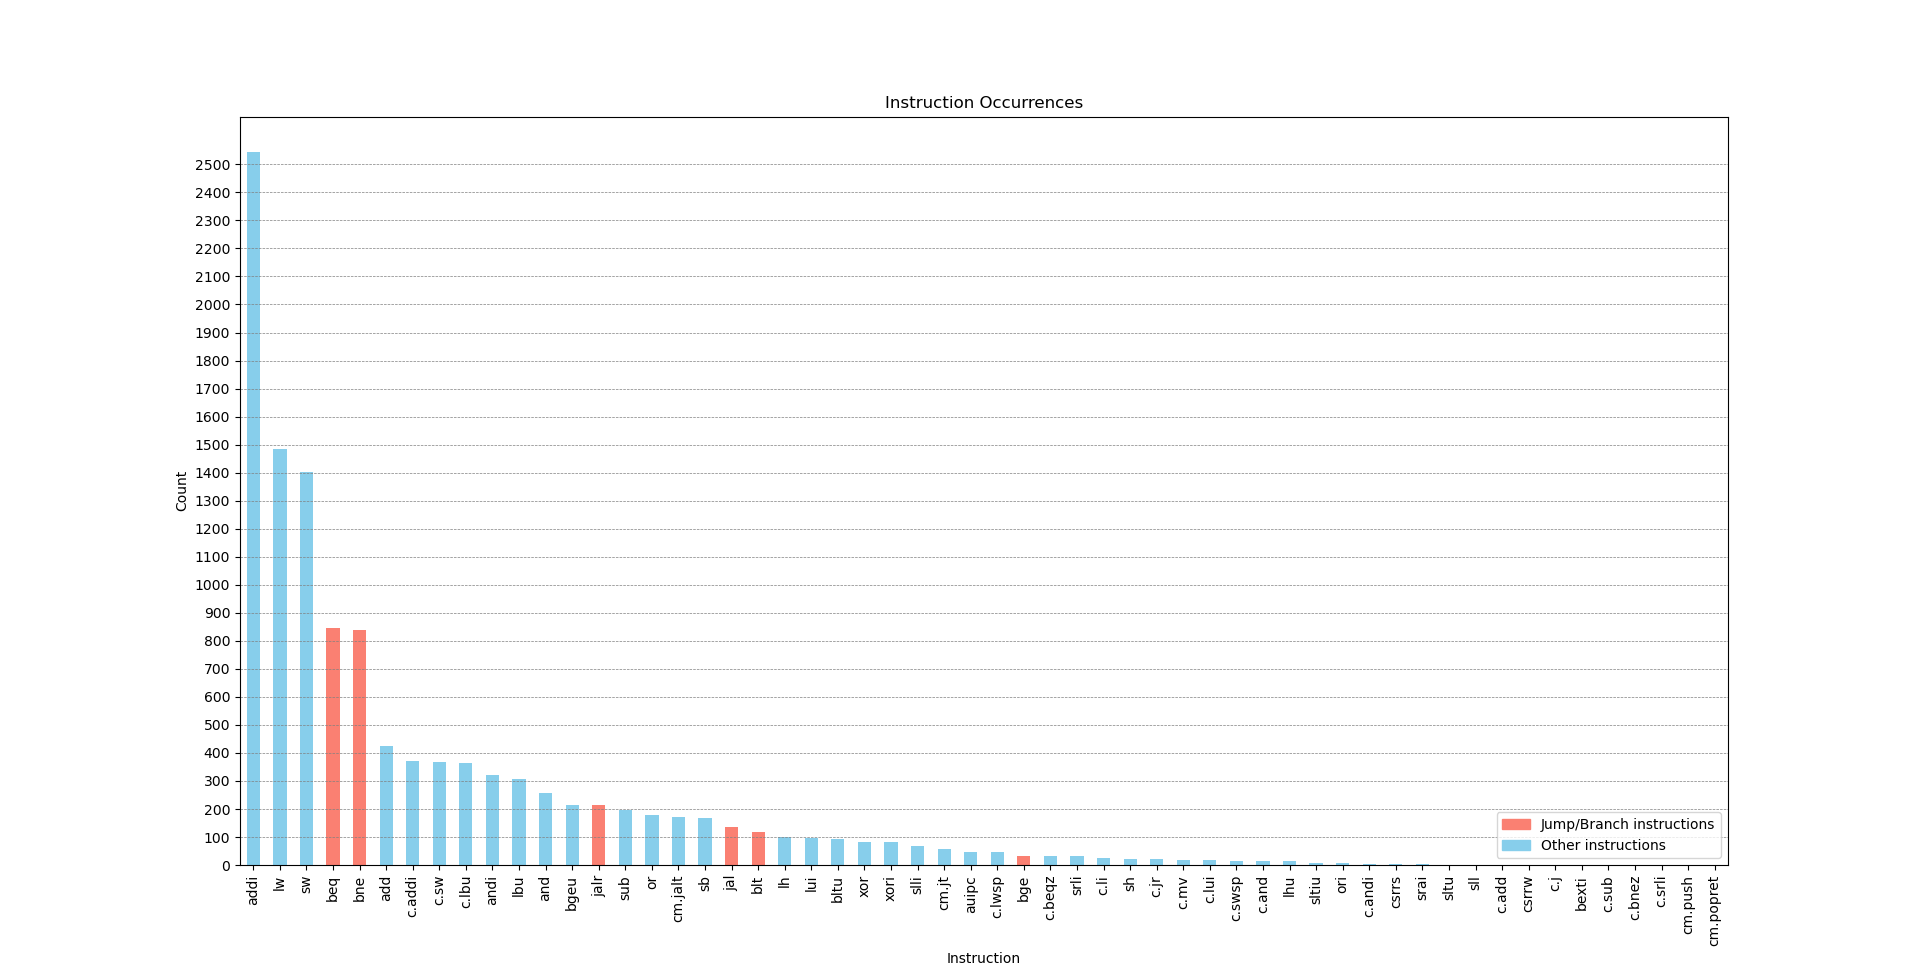
\includegraphics[width=\textwidth]{docs/images/instruction_occurances_all_legend.png}
%     \caption{All instructions in the generated assembly for the \textit{hello-world}\autoref{app:helloworldC} example, and the amount of calls for each instruction.}
%     \label{fig:instr_occ}
% \end{figure}


% \section{Limitations of glitch protection}
% \label{sec:limits}

% Despite greatly increasing the hardware security of devices, many glitch protection methods can have some common limitations. For instance the coverage of protection can often be incomplete. This means that designers often only focus on the most critical glitches, and can therefore sometimes overlook seemingly insignificant glitches that might break the system. For instance, a designer could implement a robust check to see whether the program counter has been modified during execution. However if an attacker glitches the program counter on boot, it could go undetected by the checker mechanism. 

% In general, glitch protection mechanisms will add to both the area and power consumption of a chip. Often the added area also comes from components that are logically redundant. In addition there will potentially be quite a lot of latency added. As previously described in \autoref{sec:xsecure}, the \textit{PC-hardening} module will add one extra cycle per jump or branch that is not taken. From \autoref{fig:instr_occ} it can be seen that even in a very simple program the potential for added latency is big. However, most of the potential performance gain that can be achieved from removing the \textit{Xsecure} features is mitigated by the side-channel safety features, which can not be removed. 

% From simulation and synthesis of both cores it is obvious that the argument for using a dual-core lockstep mechanism cannot be made solely on resource usage and performance gain alone. However, the main advantage will be the coverage and robustness gained. To test this claim, the regular and dual-core setups will both be subjected to several different glitch attacks that will take place in different parts of the pipeline. The quality of the solution will then be determined by how effective each setup is at responding to the attack. 

\section{Problem Definition}
\label{sec:problem_definition}

The \textit{OpenHW} group has developed the CV32E40S core which focuses on secure operation. A feature of this core is the ISE \textit{Xsecure} which introduces ways of mitigating side-channel attacks as well as glitch attacks. To stop glitch attacks the extension introduces features like ECC, CSRH and PCH that cover specific parts of the core. These can increase excution time, area and power usage of the core. This project investigates the possibility replacing these pre-existing security features in favour of using dual RISC-V cores in a lockstep mechanism. This will come at the cost of increased area and power usage. However, by continuously comparing all inputs and outputs of the two cores, we can achieve a greater level of fault coverage and robustness. 

To investigate the feasibility of the \textit{CV32E40DC} both cores will be synthesized and their PPA will be compared. In addition both will be tested against simulations of possible glitch attacks. The quality of our proposed architecture is determined by the ability to detect glitch attacks. The ability to fix the glitch or reset the core upon detection of a glitch is not investigated. This is because such things are handled by different parts of the system. PPA also plays a role in determining the quality of our solution. However, as the core is meant to be used in secure operations we allow an increase in power and area in favour of robustness. 
